\documentclass[tikz,border=6pt]{standalone}
% Native vector figure style. Okabe-Ito-derived colors; labels remain readable
% without color. Figure meaning must never depend on color alone.
\usepackage[T1]{fontenc}
\usepackage{helvet}
\renewcommand{\familydefault}{\sfdefault}
\hyphenpenalty=10000
\exhyphenpenalty=10000
\usepackage{tikz}
\usetikzlibrary{arrows.meta,positioning,fit,backgrounds,calc}
\definecolor{paBlue}{HTML}{0072B2}
\definecolor{paOrange}{HTML}{E69F00}
\definecolor{paGreen}{HTML}{009E73}
\definecolor{paPurple}{HTML}{CC79A7}
\definecolor{paInk}{HTML}{263441}
\tikzset{
  block/.style={draw=paInk,line width=.65pt,rounded corners=2pt,
    align=center,text=paInk,font=\sffamily\fontsize{9}{11}\selectfont,
    minimum height=1.15cm,text width=3.0cm,inner sep=5pt,fill=white},
  cpu/.style={block,fill=paBlue!10},
  memory/.style={block,fill=paOrange!13},
  compute/.style={block,fill=paGreen!10},
  control/.style={block,fill=paPurple!12},
  link/.style={-{Latex[length=2mm]},draw=paInk,line width=.8pt},
  duplex/.style={{Latex[length=2mm]}-{Latex[length=2mm]},draw=paInk,line width=.8pt},
  streaming/.style={duplex,draw=paBlue,line width=1.15pt},
  boundary/.style={draw=paInk!65,dashed,line width=.65pt,rounded corners=4pt},
  note/.style={font=\sffamily\fontsize{8}{10}\selectfont,align=center,text=paInk},
}

\begin{document}
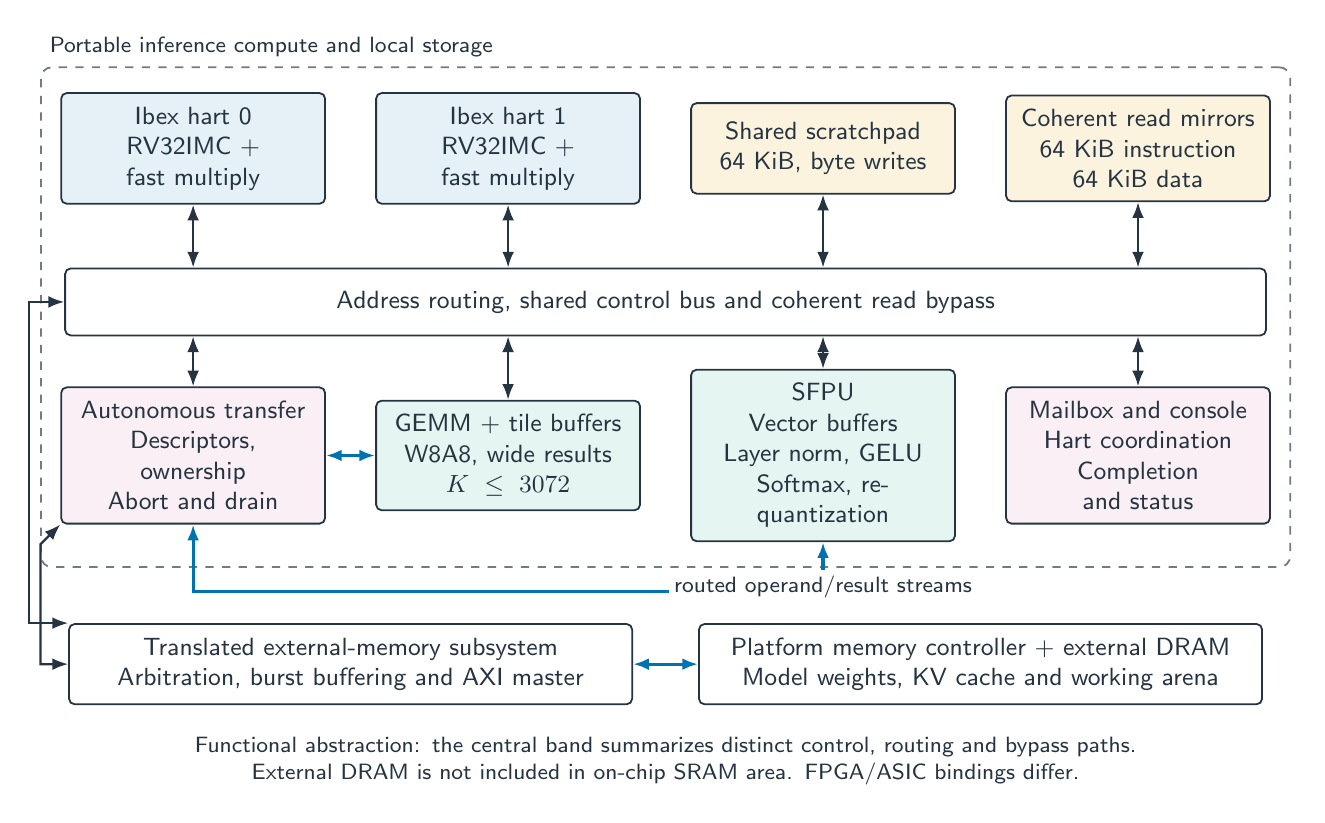
\begin{tikzpicture}[x=1cm,y=1cm]
  \node[cpu] (h0) at (1.8,6.8) {Ibex hart 0\\RV32IMC + fast multiply};
  \node[cpu] (h1) at (5.8,6.8) {Ibex hart 1\\RV32IMC + fast multiply};
  \node[memory] (ram) at (9.8,6.8) {Shared scratchpad\\64 KiB, byte writes};
  \node[memory] (mirrors) at (13.8,6.8) {Coherent read mirrors\\64 KiB instruction\\64 KiB data};
  \node[block,text width=14.9cm,minimum height=.85cm] (fabric) at (7.8,4.85)
    {Address routing, shared control bus and coherent read bypass};
  \foreach \n in {h0,h1,ram,mirrors} {
    \draw[duplex] (\n.south) -- (\n.south |- fabric.north);
  }
  \node[control] (transfer) at (1.8,2.9) {Autonomous transfer\\Descriptors, ownership\\Abort and drain};
  \node[compute] (gemm) at (5.8,2.9) {GEMM + tile buffers\\W8A8, wide results\\$K\leq3072$};
  \node[compute] (sfpu) at (9.8,2.9) {SFPU\\Vector buffers\\Layer norm, GELU\\Softmax, requantization};
  \node[control] (io) at (13.8,2.9) {Mailbox and console\\Hart coordination\\Completion and status};
  \foreach \n in {transfer,gemm,sfpu,io} {
    \draw[duplex] (fabric.south -| \n.north) -- (\n.north);
  }
  \draw[streaming] (transfer.east) -- (gemm.west);
  \draw[streaming] (transfer.south) -- ++(0,-.85) -|
    node[note,pos=.55,fill=white,inner sep=2pt] {routed operand/result streams} (sfpu.south);
  \node[block,text width=6.8cm,minimum height=.95cm] (axi) at (3.8,.25)
    {Translated external-memory subsystem\\Arbitration, burst buffering and AXI master};
  \draw[duplex] (transfer.south west) -- ++(-.25,-.25) |- (axi.west);
  \draw[duplex] (fabric.west) -- ++(-.45,0) |- (axi.north west);
  \node[block,text width=6.8cm,minimum height=.95cm] (external) at (11.8,.25)
    {Platform memory controller + external DRAM\\Model weights, KV cache and working arena};
  \draw[streaming] (axi.east) -- (external.west);
  \begin{scope}[on background layer]
    \node[boundary,fit=(h0)(h1)(ram)(mirrors)(fabric)(transfer)(gemm)(sfpu)(io),
      inner xsep=7pt,inner ysep=9pt] (core) {};
  \end{scope}
  \node[note,anchor=south west] at (core.north west) {Portable inference compute and local storage};
  \node[note,anchor=north,text width=15.8cm] at (7.8,-.55)
    {Functional abstraction: the central band summarizes distinct control, routing and bypass paths.\\
     External DRAM is not included in on-chip SRAM area. FPGA/ASIC bindings differ.};
\end{tikzpicture}
\end{document}
